\documentclass[a4paper]{article}

%% Language and font encodings
\usepackage[english]{babel}
\usepackage[utf8x]{inputenc}
\usepackage[T1]{fontenc}

%% Sets page size and margins
\usepackage[a4paper,top=2.54cm,bottom=2.54cm,left=2.54cm,right=2.54cm,marginparwidth=1.75cm]{geometry}

%% Useful packages

\usepackage{graphicx}
\usepackage[colorinlistoftodos]{todonotes}
\usepackage[colorlinks=true, allcolors=blue]{hyperref}
\usepackage{amsmath, amsthm, amssymb}
\newtheorem{prop}{Proposition}
\usepackage{float}
\usepackage{ragged2e}
\usepackage{subcaption}
\usepackage{hanging}
\usepackage{algorithm}
\usepackage{algcompatible}
\title{Object Detection for Body-worn Video}
\author{Carson Hu, Jaydeep Singh, Mingxi Sun, Kan Yao, Duo Zhang}

\begin{document}
\maketitle
\nocite{*}


\begin{abstract}
This paper applies Faster-RCNN, a neural-network based object detection algorithm, to the field of Body-worn video: we want to differentiate between police and non-police individuals. Along with creating a functional object detector, we want to improve the results of Faster-RCNN. We first manually prepare and label the training data, and apply repair and superresolution techniques to the images to increase their resolution. With regards to the network, we have tried multiple approaches to modify the loss function of Faster-RCNN to increase inter-class variance and decrease intra-class variance. Currently our results in improving the network are either unsatisfactory or incomplete, but we believe that we have made significant progress in developing a better object detection algorithm for police detection.
\end{abstract}

\section{Introduction}
Much of the current object detection literature focuses on detection for common benchmarks, such as PASCAL VOC, MNIST, and WIDER FACE. These datasets often include easily separable object classes and images of consistent quality/perspective. As a result, existing detectors are not immediately applicable to complex real-world datasets, such as police body-worn camera. Police body worn camera is often shot in a variety of image resolutions, lighting conditions, and camera/object motions, making the task of training effective detectors very difficult. \\ 
\indent
In this paper we propose a end-to-end detection pipeline capable of dealing with the unique challenges of body-worn video datasets. We aim for detection software to accurately, and in real-time, detect and distinguish between two object classes in LAPD body-worn video: police (defined as LAPD officers in uniform) and others (any individual not belonging to the police class). \\
\indent
The completed detection pipeline, which still requires hyperparameter tuning and testing, is shown in Figure \ref{pipeline} . After manual pre-processing of the data, data is fed through two image enhancement networks, the Low Dimensional Manifold Model (LDMM) and deep-learning based Neural Enhance, improving the quality and resolution of data. This data is then used as testing and training sets for a modified Faster R-CNN network, modeled off the original Caffe implementation in \cite{fasterrcnn}. \\
\indent
In this paper, we contribute to the Faster-RCNN structure with the addition of two loss functions, center loss and contrastive loss. These loss functions, building off work in \cite{Wen2016_facercnn}, promote effective separation of the deep features in feature space corresponding to the two object classes. It is believed that a proper balance of the softmax classification loss, center loss, and contrastive loss in Faster-RCNN will further improve detection mAP, but this hypothesis has not been fully tested.

\section{Dataset}
The dataset used for training and testing consists of around 700 body-worn camera videos taken from on-duty Los Angeles Police Department officers. The videos are sampled at 1 fps to yield around 1.0 million raw image frames. The LAPD dataset is rife with image defects, complicating the object detection task beyond existing detection benchmark sets. Typical defects include those arising from camera motion, object motion, variable environmental lighting, poor camera quality, and heavy occlusion (from background and from other object classes). Typical challenging examples are shown in Figure \ref{fig:defects} below.

In the following sections, the pipeline for data pre-processing is discussed. 

\subsection{Data Annotation}
We first filter from the original 1 million raw frames those containing members of either object class, with preference towards those of higher quality and distinguishable objects. These preferences are aimed towards improving training, and minimizing sources for error in bounding box annotation. Using an open source software LabelImg \cite{github1}, we annotate each object with a class label, and bounding box circumscribing as much of the object as appears in frame. After a verification process enforcing uniform bounding box standards, this process yields a dataset of 72591 frames with annotations. This dataset comprises our training set, and we assume it to be fairly representative of typical image features/defects present in body-worn video.

\begin{figure}[H]
\begin{subfigure}{.33\textwidth}
	\centering	
    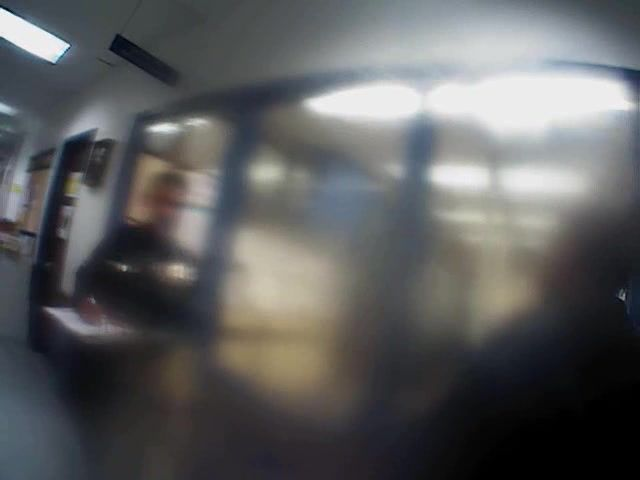
\includegraphics[width=.8\linewidth]{blur_censored.jpg}
    \caption{Camera Blur}
    \label{fig:sfig1}
\end{subfigure}%
\begin{subfigure}{.33\textwidth}
	\centering
    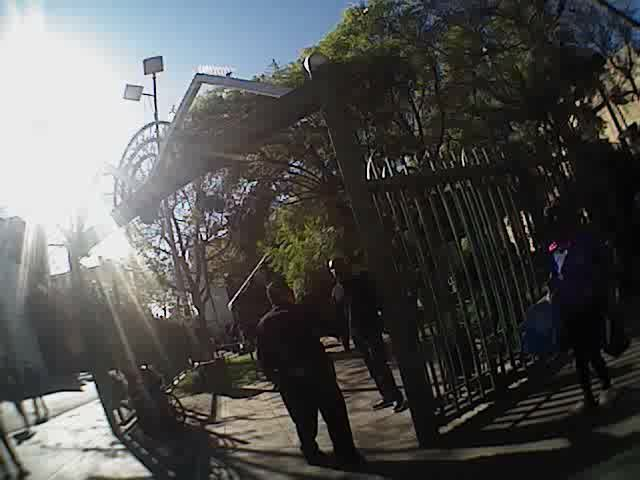
\includegraphics[width=.8\linewidth]{bright_censored.jpg}
	\caption{Variable Natural Lighting}
    \label{fig:sfig2}
\end{subfigure}
\begin{subfigure}{.33\textwidth}
	\centering
    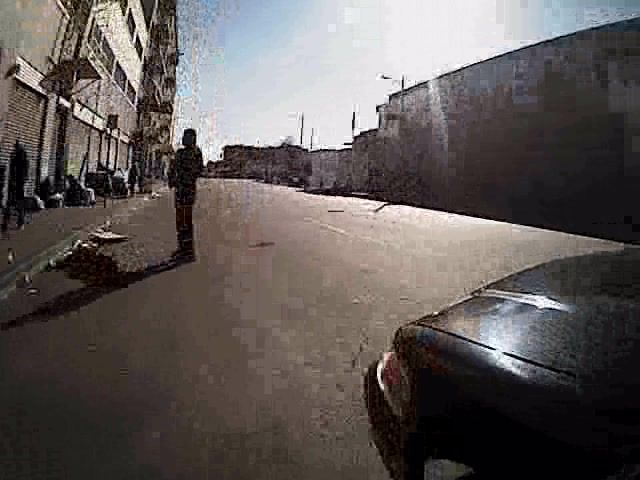
\includegraphics[width=.8\linewidth]{lowres_censored.jpg}
	\caption{Low Resolution}
    \label{fig:sfig3}
\end{subfigure}
\begin{subfigure}{.33\textwidth}
	\centering
    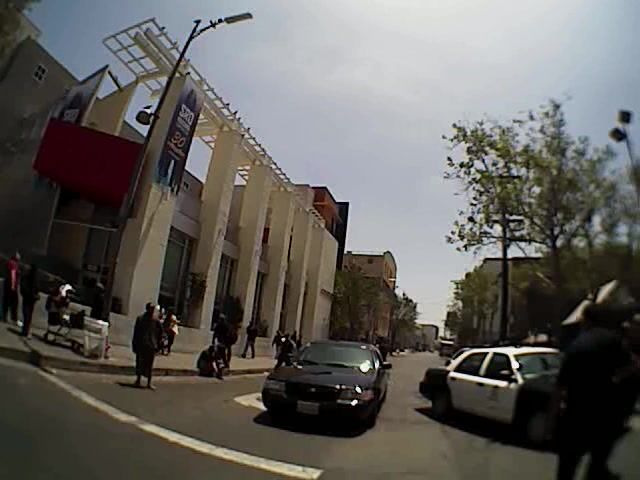
\includegraphics[width=.8\linewidth]{depth_censored.jpg}
	\caption{Variable Object Depth}
    \label{fig:sfig4}
\end{subfigure}
\begin{subfigure}{.33\textwidth}
	\centering
    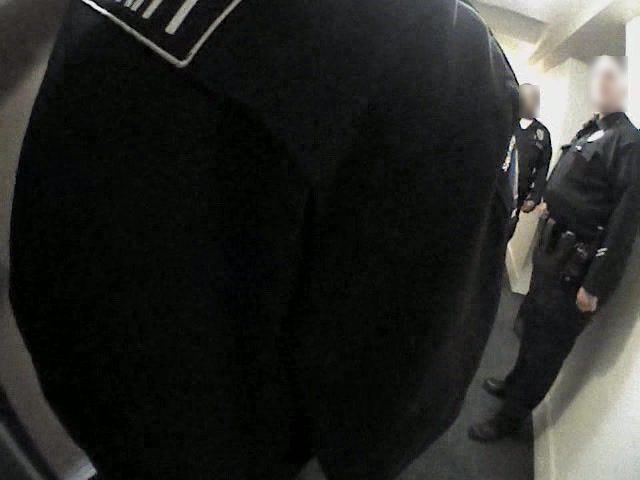
\includegraphics[width=.8\linewidth]{occlusionnew_censored.jpg}
	\caption{Object Occlusion}
    \label{fig:sfig5}
\end{subfigure}
\begin{subfigure}{.33\textwidth}
	\centering
    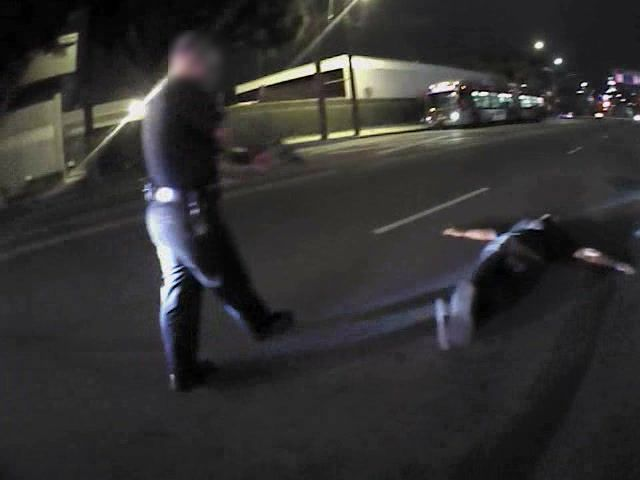
\includegraphics[width=.8\linewidth]{pose_censored.jpg}
	\caption{Variable Object Pose}
    \label{fig:sfig6}
\end{subfigure}
\caption{Typical Image Defects}
\label{fig:defects}
\end{figure}



\section{Deep Learning Method}
We first try to apply an existing Deep Learning Method called Faster-RCNN\cite{fasterrcnn} on our dataset. By learning a mapping from the high dimensional pixel space of image frames to the outputs (bounding box coordinates and classification labels), deep learning algorithms allow the computer to optimize over potential models, parameterized by high dimensional weight vectors. We use large training sets, with ground-truth labels and bounding boxes, to minimize a loss function and arrive at the optimal detection algorithm.
\subsection{Faster-RCNN}
Faster-RCNN\cite{fasterrcnn} is the most popular object detection algorithm. Compared to other available methods, Faster-RCNN not only achieves the highest detection accuracy on the benchmark set, but also reduces the runtime by $25$ to $50\%$ compared to Fast-RCNN\cite{fastrcnn}. Faster-RCNN  trains the model to approximate a classification function of deep features by using different layers of non-linear functions to approximate a network. It is a state-of-the-art object detection network which depends on region proposal algorithms (RPN) to hypothesize object locations.\\
\begin{figure}[H]
\begin{center}
\begin{tabular}{c}
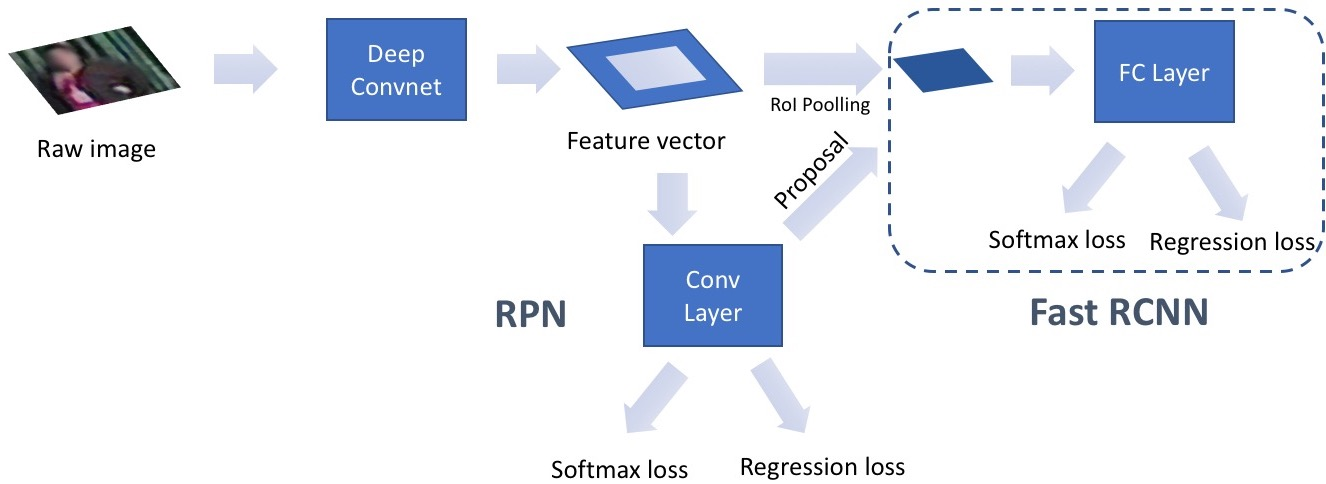
\includegraphics[width=1.0\textwidth]{Fasterpipeline.jpg}\\
\end{tabular}
\end{center}
\caption{Faster RCNN structure.}
\label{structure}
\end{figure}

After pre-processing the image by convolution, the network first transfers the data to the RPN layer for training. The RPN stage will first give approximately 2000 different region proposals for each image and then train the network to determine whether these regions belong to the foreground or background by comparing them with ground truth. After that the RPN stage will send the proposed region of foreground to Fast RCNN layer. The Fast RCNN stage trains the network to determine the labels of different regions by minimizing the loss of the classification function using the training set.
\subsection{Experiment}
In our experiment on the body-worn dataset, We apply the Faster-RCNN \cite{fasterrcnn} algorithm twice. Here is our network structure:
\begin{align*}
& \textbf{Stage 1 RPN}\\
& \textbf{Stage 1 Fast RCNN}\\
&\textbf{Stage 2 RPN}\\
& \textbf{Stage 2 Fast RCNN}\\
\end{align*}
During the first stage, we create the RPN layer from scratch and use the output of Stage 1 RPN to initialize the first Fast RCNN layer. Right now these two networks do not share any convolution layers. After we finish the first Faster-RCNN algorithm, we will use the output of Stage 1 Fast RCNN to initialize the RPN layer again. We only fine-tune layers unique to the RPN layer so that now the Fast RCNN share convolution layers with RPN layer. Finally we can unify a network for object detection. We run each RPN stage for 80000 iterations and run each Fast-RCNN stage for 40000 iterations.

\subsection{Primary Results}\label{subsec:primary_result}
There are many successful networks provided by Faster-RCNN \cite{fasterrcnn}. In our experiment, we train our dataset on both the ZF net (which contains 5 convolution layers) and VGG16 net (which contains 16 convolution layers).\\

To measure the accuracy, we will use the notions of AP (Average Precision) and MAP (Mean Average Precision). When pre-processing the images we split a test set. We set the test set to be 20\% of the whole dataset which contains 14000 images according to our dataset. After the training, we apply the network on the test set to generate proposed regions for different labels. We compute the overlap area of each region with the ground truth. If the overlap area is greater than 70\% of the whole area, we will consider the proposed region as a correct detection. The Average Precision AP is the accuracy rate of each label(\textit{police} and \textit{others}) and the Mean Average Precision MAP is the mean value of the accuracy rate of different labels.\\

Here is the result of our dataset:
\begin{itemize}
\item{\bf ZF(5 convolution ayers):}
\begin{itemize}
\item Police: 0.864
\item Others: 0.828 
\item MAP: 0.846
\end{itemize}
\item{\bf VGG(16 convolution layers):}
\begin{itemize}
\item Police: 0.888
\item Others: 0.873
\item MAP: 0.881
\end{itemize}
\end{itemize}
The police always have a better detection accuracy than \textit{others} as they tend to share same features and their intra-class variation is small.\\
\subsection{Detection Example}
\begin{figure}[H]
\centering
\begin{minipage}{\textwidth}
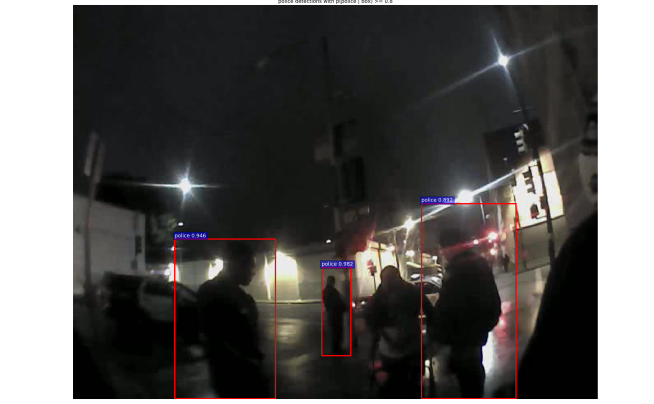
\includegraphics[width=0.5\textwidth]{Detect_Police.png}
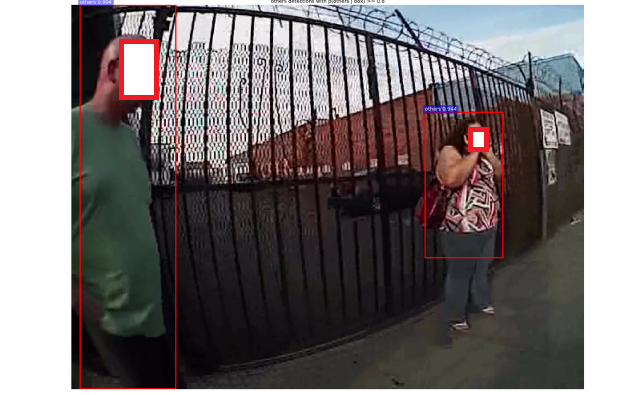
\includegraphics[width=0.5\textwidth]{Detect_Others.png}\\
\footnotesize{The left figure is a detection example for \textit{police} and the right figure is a detection example for \textit{others} \par}
\caption{Detection examples}
\label{Detection}
\end{minipage}
\end{figure}

\subsection{Detection Problem}
Although the detection result seems to be good, we still have much room for improvement. Here are some examples:\\
\begin{figure}[!ht]
\begin{center}
\begin{tabular}{c}
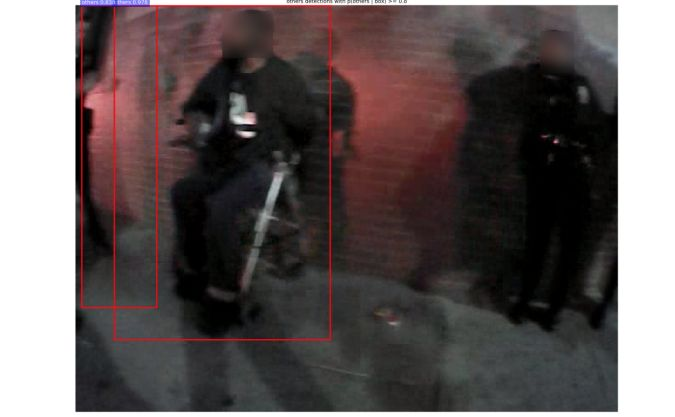
\includegraphics[width=0.5\textwidth]{Wrong_Detection_censored_two.jpg}\\
\end{tabular}
\end{center}
\caption{Wrong Detection.}
\label{lowresolution}
\end{figure}

\begin{figure}[H]
\begin{center}
\begin{tabular}{c}
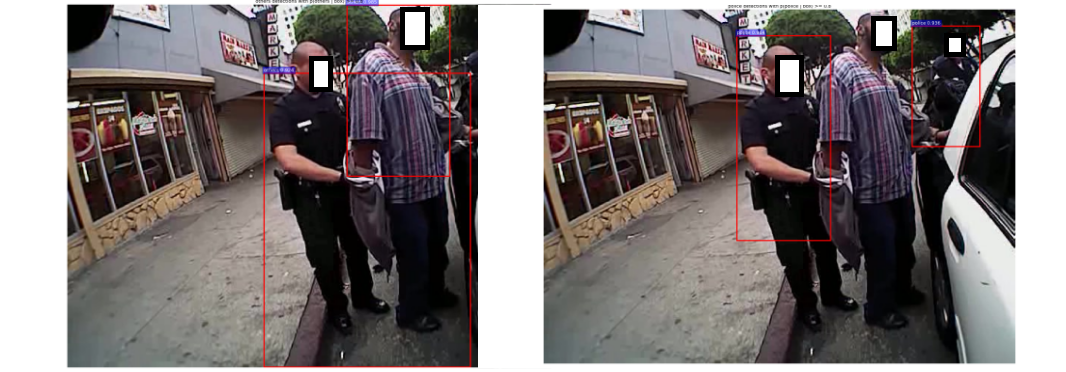
\includegraphics[width=1.1\textwidth]{Duplicate_Detection.png}\\
\end{tabular}
\end{center}
\caption{Duplicated detection.}
\label{duplicates}
\end{figure}

\begin{figure}[H]
\begin{center}
\begin{tabular}{c}
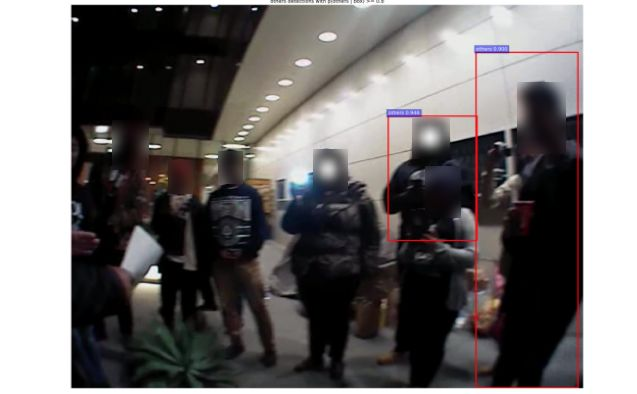
\includegraphics[width=0.5\textwidth]{Missing_Detection_censored.jpg}\\
\end{tabular}
\end{center}
\caption{Missing objects in multiple objects image.}
\label{missing}
\end{figure}
%\begin{figure}[H]
%\centering
%\begin{minipage}{\textwidth}
%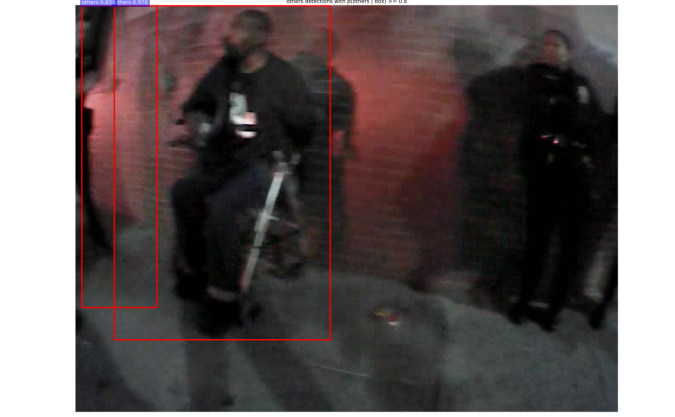
\includegraphics[width=0.5\textwidth]{Wrong_Detection.png}
%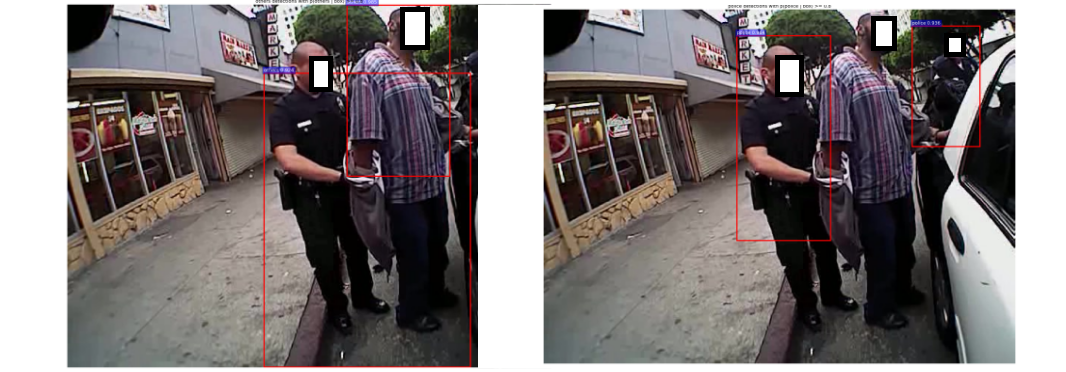
\includegraphics[width=0.5\textwidth]{Duplicate_Detection.png}\\
%\footnotesize{The figure left shows an example of wrong detection as it bounds an arbitrary thing. The figure left shows an example of Duplicate detection. The network bounds the same target several times \par}
%\caption{Detection failure}
%\label{Detection}
%\end{minipage}
%\end{figure}
\subsection{Improvement Strategy}
We find that the errors of our detection are strongly related to the low resolution of our dataset and the intra-class differences, especially for \textit{others}, as their deep features may vary a lot. To solve these problems, our research focus on these two approaches:
\begin{itemize}
\item { Improve image quality.}
\item { Improve loss functions.}
\end{itemize}
We will discuss these two approaches in the following sections.

\section{Image Enhancement}
To improve the performance of our network, we apply image enhancement techniques on the dataset. First, we repair the images using a low-dimensional manifold model (LDMM) which allows us to extract better features from low quality images. Then we use neural-network based superresolution techniques to upscale the images to 4 times their original size.

\subsection{LDMM}
The problem of image reconstruction is represented as $z = \Phi_I f + \epsilon$, where $z$ is the observed image. The operator $\Phi_I$ typically does some damage to the image such as blurring or down-sampling. $f \in \mathbb{R}^{m \times n \times 3}$ is the "original" noiseless image in RGB we want to recover and $\epsilon$ is the noise. Recovering $f$ from $z$ is inherently ill-posed. Recently, a low-dimensional manifold model (LDMM) has been proposed and achieved state-of-the-art performances in tasks such as image reconstruction with significant missing information \cite{ldmmimageprocessing} \cite{ldmmhyperspectral}. The authors assume that the patch set of an image samples a smooth low-dimensional manifold and use the dimension of the manifold as regularization. Then the optimization problem is solved by alternating minimization with respect to the image and the manifold. We hereby introduce the main idea and implementation of LDMM.\cite{nonlocallaplacian}

\subsubsection{Patch Manifold}
Consider an image $f \in \mathbb{R}^{m \times n \times 3}$. For any pixel $(i,j) \in \{1,...,m\}\times\{1,...n\}$, let a \textbf {patch} $p_{ij} \in \mathbb{R}^{s_1 \times s_2 \times 3}$ be the cube of size $s_1 \times s_2 \times 3$ with $(i,j,k), ~ ~k\in\{1,2,3\}$ in the upper left corner of the cube. The patch set is the collection of all the patches. 
\begin{align}
\mathcal{P}(f) = \{P_{ij} : (i,j) \in \{1,...,m\} \times \{1,...,n\} \} \subset \mathbb{R}^d,~ ~  d = s_1 \times s_2 \times 3
\end{align}

The basic assumption of LDMM is that $\mathcal{P}(f)$ is a discrete sampling of a smooth manifold $\mathcal{M}(f) \subset \mathbb{R}^{d}$ called the \textbf{patch manifold}. For real-life images, $\mathcal{M}(f)$ is always of lower dimension than $d$. We want to recover $f$ such that the dimension of $\mathcal{M}(f)$ is as small as possible. In other words, the goal is to solve the following optimization problem.
\begin{align}
\min_{f } \dim \mathcal{M}(f) ~ ~ \text{subject to: } z = \Phi_I f, \mathcal{P}(f) \subset \mathcal{M}(f)
\end{align}

A result from differential geometry gives us a convenient way to calculate the dimension of $\mathcal{M}(f)$.
\begin{prop}
let $\mathcal{M}$ be a smooth submanifold isometrically embedded in $\mathbb{R}^d$, for any $x\in \mathcal{M}$, \[\dim \mathcal{M} = \sum_{j=1}^{d} \| \nabla_{\mathcal{M}} \alpha_j (x) \| ^2\]
where $\alpha_j$, $j = 1,...,d $ are the coordinate functions i.e. $\alpha_j(x) = x_j$
\end{prop}
Then (2) can be transformed into the following:
\begin{align}
\min_{f } & \sum_{j=1}^{d} {\|\nabla_{\mathcal{M}} \alpha_j\|}^2_{L^2(\mathcal{M})} + \lambda \|b-\Phi_I f -\epsilon\|^2_2 ~ ~
\text{subject to: } \mathcal{P}(f) \subset \mathcal{M}(f)
\end{align}
 

We then employ numerical methods to solve (3). In \cite{PointIntegralMethod}, the authors avoid discretization the manifold gradient operator $\nabla_{\mathcal{M}}$ by the point integral method. This method involves solving $d$ linear equations per iteration, thus is very computationally expensive, especially for our large dataset. We instead implement the Weighted Graph Laplacian (WGL) \cite{nonlocallaplacian} to discretize $\nabla_{\mathcal{M}}$.
%The LDMM extracts a patch manifold, a lower dimension representation of the image, and aims to minimize the dimension of that patch manifold. This patch manifold can help to find $f$ using methods like the Point Integral Method.
%anyways with LDMM you use the patch manifold to help find $f$, using stuff like the Point Integral Method.
%weight: Weight is a positive function, i.e $ w(p,q) = \exp(- \frac{\vert \vert p - q \vert \vert ^2}{\sigma^2})$ is used in this method. 

\subsubsection{Numerical Implementation}

\begin{algorithm}
\caption{LDMM for 3D scientific data reconstruction from partial sampling}
\begin{algorithmic}
\STATE \textbf{Require: } A subsampled data $f \vert_\Omega = b$
\STATE \textbf{Ensure: } Reconstructed data $f$.
\WHILE{not converge}
\STATE 1. Compute the patch set $\mathcal{P}(f^k)$ from the current iterate $f^k$.
\STATE 2. Compute the weight function 
\begin{equation}
\bar{w}(x,y) = w(\mathcal{P}f^k(x), \mathcal{P}f^k(y)), ~ ~ x, y \in \bar{\Omega}
\end{equation}
\STATE 3. Assemble the new weight function
\begin{equation}
\tilde{w}(x,y) = \sum_{i=1}^d \bar{w}(x_{\widehat{1-i}},y_{\widehat{1-i}})
\end{equation}
\STATE 4. Update the data $f^{k+1}$ by solving variable $v$ in the equation
\begin{equation}
(2 \tilde{L}_{11} + (\mu - 1) \Delta) v = (\mu + 1) \tilde{W}_{12} b
\end{equation}
\STATE 5. $k \gets k + 1$
\ENDWHILE
\STATE $f = f^k$
\end{algorithmic}
\end{algorithm}

\begin{enumerate}
\item Since $f^k$ is an image, we can construct the patch set from the current $f^k$.

\item The weight function between two points is constructed by mapping each point to its corresponding patch and taking the weight between these two patches. The weight can be any weight function, but we use $ w(p,q) = \exp(- \frac{\vert \vert p - q \vert \vert ^2}{\sigma^2})$.

\item $x_{\hat{j}}$ is the $j$'th element after $x$ in the patch. The new weight function $\tilde{w}(x,y)$ is found by summing up the weights of the $d$ elements before $x$ and $y$ in their respective patches. So it iterates over every element in each patch.

\item \begin{itemize}
\item $\tilde{W}$ is the weight matrix constructed with weight function $\tilde{w}$ calculated on every pair of points. $\tilde{W}_{12}$ is a block matrix corresponding to the sampled points.
\item $\tilde{D}$ is the diagonal degree matrix s.t $\tilde{D}(x,x) = \sum\limits_{y \in \bar{\Omega}} \tilde{w}(x,y)$
\item Then, $\tilde{L} = \tilde{D} - \tilde{W}$, the weighted Graph Laplacian. $\tilde{L}_{11}$ is a block matrix of $L$ corresponding to the unsampled points.
\item $\Delta$ is a diagonal matrix with diagonal entries equaling the sum of the rows of $\tilde{W}_{12}$.
\item $v$ and $b$ are vectors corresponding to the unsampled and sampled portions of image $f$.
\item $\mu$ is equal to the number of points divided by the number of sampled points.
\end{itemize}

By solving for $v$, one can construct $f^{k+1}$ by combining $v$ and $b$. This converges to the repaired image.

\end{enumerate}

\subsubsection{Results}


LDMM repair does an excellent job at restoring images with very low quality especially in terms of removing tile effect, as can be seen from these examples.

\begin{figure}[H]
\begin{minipage}[b]{0.12\textwidth}
 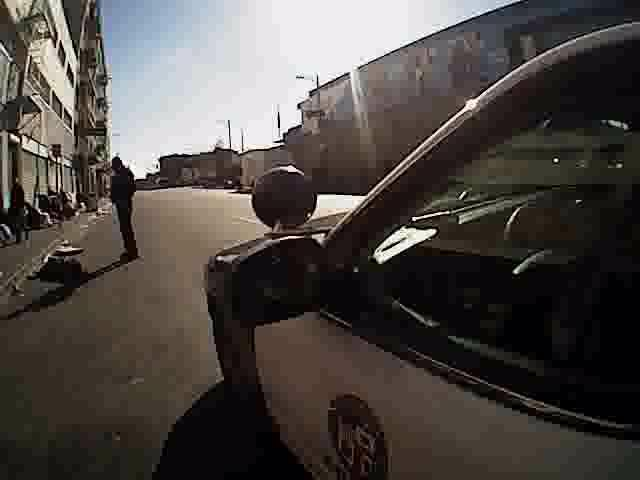
\includegraphics[trim=0 7cm 21cm 6cm, clip, width=\textwidth]{original3.jpg}
 \caption{Original Image}
 \end{minipage}
  \begin{minipage}[b]{0.12\textwidth}
    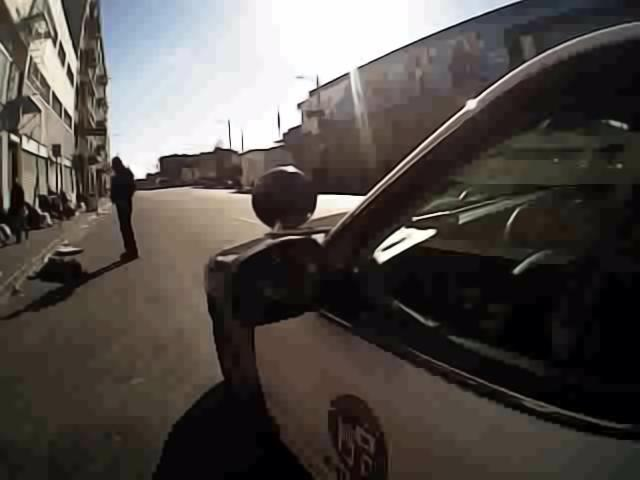
\includegraphics[trim=0 7cm 21cm 6cm, clip, width=\textwidth]{original3Repaired.jpg}
    \caption{Repaired Image}
  \end{minipage}
    \hfill
  \begin{minipage}[b]{0.12\textwidth}
 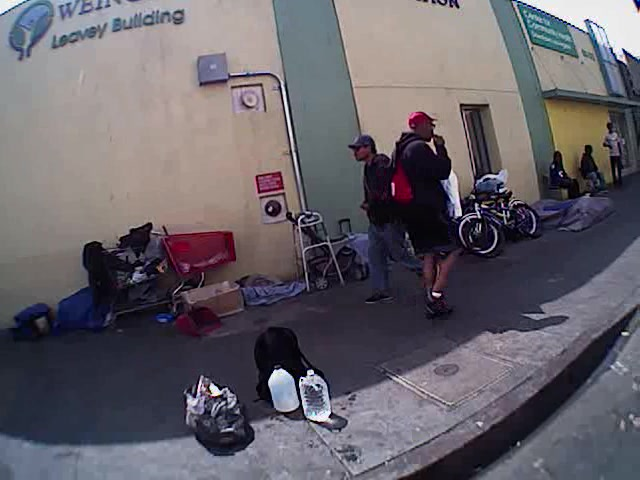
\includegraphics[trim=13.5cm 5cm 5.5cm 3cm, clip, width=\textwidth]{00253_112.jpg}
 \caption{Original Image}
 \end{minipage}
  \begin{minipage}[b]{0.12\textwidth}
    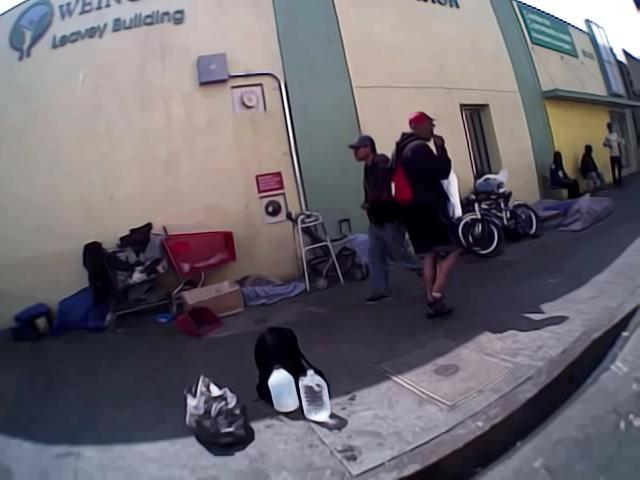
\includegraphics[trim=13.5cm 5cm 5.5cm 3cm, clip, width=\textwidth]{00253_112R.jpg}
    \caption{Repaired Image}
  \end{minipage}
  \hfill
  \begin{minipage}[b]{0.12\textwidth}
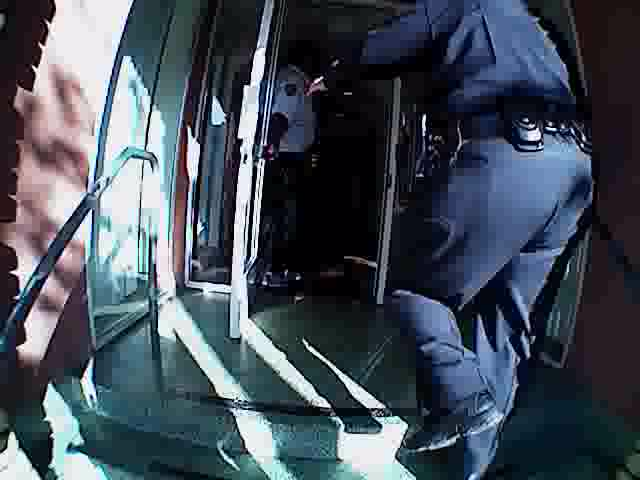
\includegraphics[trim=7.5cm 4cm 10cm 0cm, clip, width=\textwidth]{00181_29.jpg}
 \caption{Original Image}
 \end{minipage}
  \begin{minipage}[b]{0.12\textwidth}
    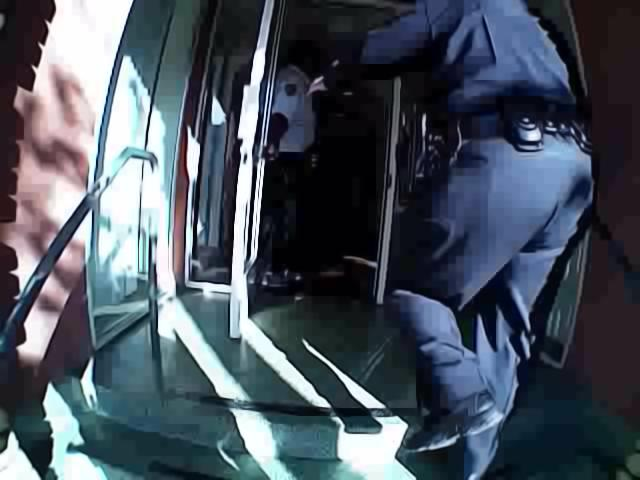
\includegraphics[trim=7.5cm 4cm 10cm 0cm, clip, width=\textwidth]{00181_29R.jpg}
    \caption{Repaired Image}
  \end{minipage}
  \hfill
\end{figure}

\subsubsection{Contrast Adjustment}

Along with the LDMM, we also adjust the image intensity values so that 1\% of the data is saturated at low and high densities. This increases the contrast of the image, allowing dark images to be easier to interpret.

\begin{figure}[H]
\begin{minipage}[b]{0.48\textwidth}
 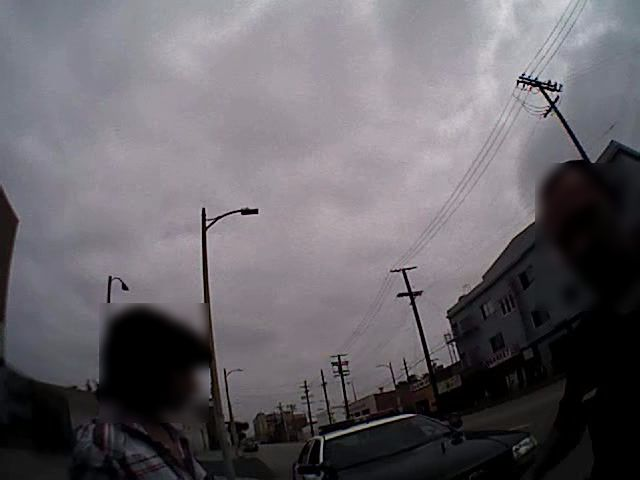
\includegraphics[width=\textwidth]{contrastee_censored.jpg}
 \caption{Original Image}
 \end{minipage}
  \hfill
  \begin{minipage}[b]{0.48\textwidth}
    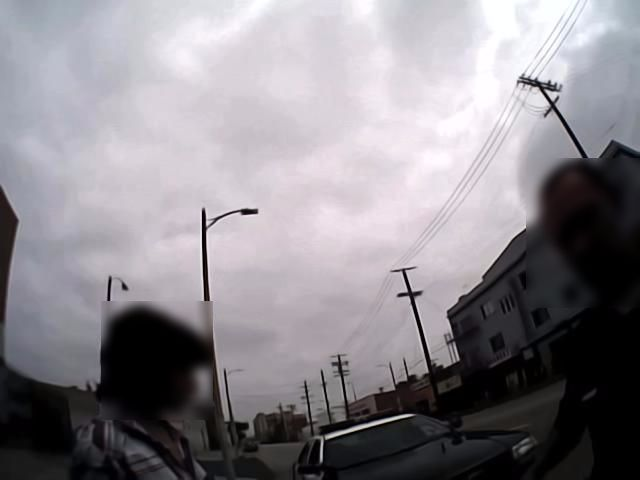
\includegraphics[width=\textwidth]{contrasted_censored.jpg}
    \caption{Repaired Image}
  \end{minipage}
\end{figure}

\subsection{Super Resolution}
\justify
LDMM techniques are sufficient to repair most image artifacts, but to boost network performance further, we try increasing the resolution of the images themselves. If $I^{LR}$ is a given low resolution image, the problem of directly inferring an upscaled (called ``super resolved") image $I^{SR}$ is referred to as single image super resolution (SISR). SISR relies on the assumption that $I^{LR}$ is downscaled from a high resolution $I^{HR}$ lying on a natural image manifold; however, the ground truth $I^{HR}$ is certainly non-unique, suggesting SISR is ill-posed. 
\subsubsection{Perceptual Loss}

As described in \cite{Perceptual}, common deep-learning approaches to SISR promote per-pixel similarity between $I^{HR}$ and the generated $I^{SR}$ by training a neural network to minimize the following mean squared error, given a training set of high resolution images $I^{HR}$ of dimension $rW \times rH \times C$, and downsampled images $I^{LR}$ of dimension $W \times H \times C$:
$$l^{SR}_{MSE} = \frac{1}{r^2WH}\sum_{x=1}^{rW}\sum_{y=1}^{rH}(I^{HR}_{x,y}-G_{\theta_g}(I^{LR})_{x,y})^2$$
Here $G_{\theta_g}$ is the output of the network on the low resolution input, parameterized by weights $\theta_g$.
While this approach improves resolution compared to non-deep learning based interpolation methods, the authors of \cite{Perceptual} observe that it neglects perceptual similarities between training set images and downsampled versions. Instead, they observe that CNNs pre-trained on image classification tasks effectively learn this valuable semantic information about the natural image manifold, storing this information in hidden layers of the network. To replace MSE loss the authors define a perceptual loss function, in which a weighted sum of hidden layer outputs from a pre-trained deep VGG-19 serves as a ``learned" loss function tailored to image classification. The loss is given below: 

$$l^{SR}_{VGG/i,j} = \frac{1}{W_{i,j}H_{i,j}}\sum_{x=1}^{W_{i,j}}\sum_{y=1}^{H_{i,j}}(\phi_{i,j}(I^{HR})_{x,y} - \phi_{i,j}(G_{\theta_G}(I^{LR}))_{x,y})^2
$$

where $W_{i,j},H_{i,j}$ are the dimensions of the feature maps of the VGG network, $\phi_{i,j}$ the  output of the feature map of the VGG network after the j-th convolution layer, and before the i-th max pooling layer, and $G_{\theta_G}(I^{LR})$ again denotes the super resolved image output.
\subsubsection{Generative Adversarial Network Techniques}
A further boost to SISR performance comes by employing Generative Adversarial Networks (GAN) into the SISR pipeline. As described in \cite{PerceptualGAN}, GAN architectures introduce a ``discriminator" network $D_{\theta_g}$ alongside the original SISR ``generative" network $G_{\theta_g}$. By alternating training of the discriminator and generator, the following min-max problem is effectively solved:
$$\min_{\theta_G} \max_{\theta_D} \mathrm{E}_{I^{HR} \sim p_{train}(I^{HR})}[\log(D_{\theta_D}(I^{HR})] 
	+ \mathrm{E}_{I^{LR} \sim p_{G}(I^{LR})}[\log(1-D_{\theta_D}(G_{\theta_D}(I^{LR})))]$$
    
Solving this problem amounts to maximizing the capability of the discriminator to discriminate between super resolution and high resolution images; in turn, the generator is encouraged to produce SR images lying on the natural image manifold. In \cite{PerceptualGAN}, this approach is shown to be superior to MSE methods on the SISR task, the latter encouraging simple smoothing in situations where GAN techniques correctly discern perceptually natural, sharp image features.
\subsubsection{Neural Enhance}
We employ a publicly available software, Neural Enhance \cite{github}, that combines the above two SISR techniques in an end-to-end image upscaling pipeline. Neural Enhance first pre-trains a generative network using perceptual loss alone, eventually introducing a discriminator for alternating GAN training. Even without re-training on the body-worn camera dataset, Neural Enhance is effective at resolving objects at varying depths in images from our dataset, as shown here.

\begin{figure}[H]
\centering
\begin{minipage}[b]{0.45\textwidth}
 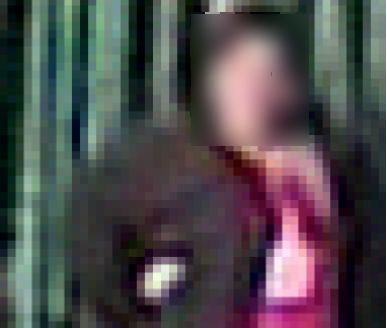
\includegraphics[width=\textwidth]{repaired_censored.jpg}
 \caption{Repaired Image}
 \end{minipage}
  \hfill
  \begin{minipage}[b]{0.47\textwidth}
    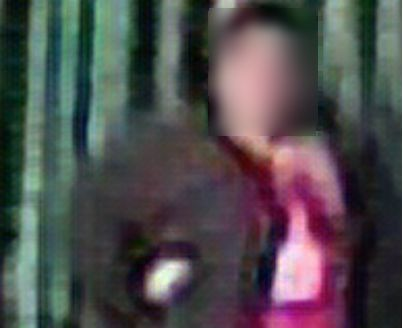
\includegraphics[width=\textwidth]{zoom1_censored.jpg}
    \caption{Enhanced Image}
  \end{minipage}
\end{figure}

\section{Loss Function Improvement}
The main goal of a deep learning algorithm is to minimize the loss function. The original Faster-RCNN uses the softmax loss function, i.e. Equation~\ref{eqn:softmax}, which maps deep features into probabilities of belonging to each class. However, for human detection, this function cannot separate features in a discriminative way as there exists huge variance in the human face and we cannot pre-collect all faces for training \cite{Wen2016_facercnn}. The primary results are shown in Section~\ref{subsec:primary_result} and we attempt to improve our loss function in order to increase the detection ability. Up to this point, we have not found an appropriate loss function that can meet our requirement. Therefore, in this section, we will mainly discuss several loss functions that we have applied and the corresponding reasons for failure. 
\begin{figure}[H]
\begin{center}
\begin{tabular}{c}
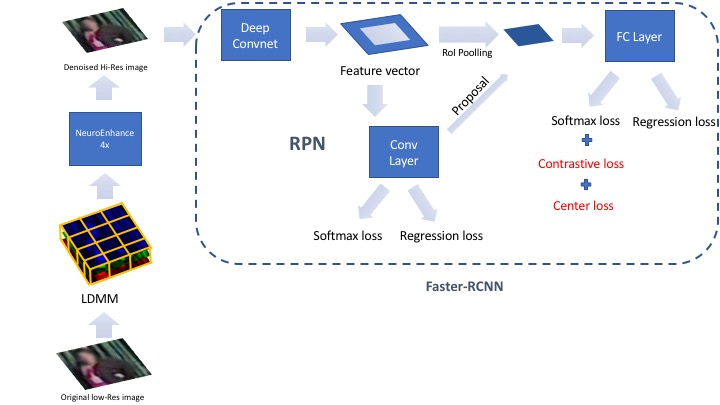
\includegraphics[width=1.0\textwidth]{pipeline_fff.jpg}\\
\end{tabular}
\end{center}
\caption{Faster RCNN structure with preprocessing and new loss functions}
\label{pipeline}
\end{figure}
\subsection{Center Loss Function}
One idea that is applicable in human detection is to minimize intra-class variance by adding a Center Loss function, i.e. Equation~\ref{eqn:center} \cite{Wen2016_facercnn}. That is, we learn a center during the training and simultaneously update the center and minimize the sum of $2$--norm distances between deep features and their corresponding centers. The overall loss function is shown in Equation \ref{eqn:centerfinal}.
\begin{equation}
\mathcal{L}_s = -\sum_{i=1}^m \log \frac{e^{W^T_{y_i}\mathbf{x}_i+b_{y_i}}}{\sum_{j=1}^n e^{W^T_{y_j}\mathbf{x}_i+b_{j}}}
\label{eqn:softmax}
\end{equation}
\begin{equation}
\mathcal{L}_c = \frac{1}{2}\sum_{i=1}^m ||\mathbf{x}_i-\mathbf{c}_{y_i}||_2^2
\label{eqn:center}
\end{equation}
\begin{equation}
\mathcal{L}=\mathcal{L}_s+\lambda \mathcal{L}_c==-\sum_{i=1}^m \log \frac{e^{W^T_{y_i}\mathbf{x}_i+b_{y_i}}}{\sum_{j=1}^n e^{W^T_{y_j}\mathbf{x}_i+b_{j}}}+\frac{\lambda}{2}\sum_{i=1}^m ||\mathbf{x}_i-\mathbf{c}_{y_i}||_2^2
\label{eqn:centerfinal}
\end{equation}
Here $\lambda$ specifies the trade-off between inter-class and intra-class variance.
The solver we use is the Stochastic Gradient Descent (SGD) for updating both center and deep features during the back-propagation. We summarize the update formulas and the learning details. 

%wrote in the functions from alg pics

\begin{align}\label{eqn:center_gradient}
\frac{\partial \mathcal{L}_C}{\partial x_i} &= x_i - c_{y_i}\\
\Delta c_j &= \frac{\sum_{i=1}^m \delta(y_i = j) \cdot (c_j - x_i)}{1 + \sum_{i=1}^m \delta(y_i = j)}
\end{align}

\begin{algorithm}[H]
\caption{The discriminative feature learning algorithm}
\hangindent=2em
\hangafter=1
\textbf{Input:} Training data $\{x_i\}$. Initialized parameters $\theta_C$ in convolution layers. Parameters $W$ and $\{c_j | j = 1, 2, \dots, n\}$ in loss layers, respectively. Hyperparameter $\lambda$, $\alpha$, and learning rate $\mu^t$. The number of iterations $t \gets 0$.

\textbf{Output:} The parameters $\theta_C$.
\begin{algorithmic}[1]
\WHILE{not converge}
\STATE $t \gets t + 1$.
\STATE Compute the joint loss by $\mathcal{L}^t = \mathcal{L}_S^t + \mathcal{L}_C^t$.
\STATE Compute the backpropagation error $\frac{\partial \mathcal{L}^t}{\partial x_i^t}$ for each $i$ by $\frac{\partial \mathcal{L}^t}{\partial  x_i^t} = \frac{\partial \mathcal{L}^t_S}{\partial x_i^t} + \lambda \cdot \frac{\partial \mathcal{L}_C^t}{\partial x_i^t}$.
\STATE Update the parameters $W$ by $W^{t+1} = W^t - \mu^t \cdot \frac{\partial \mathcal{L}^t}{\partial W^t} = W^t - \mu^t \cdot \frac{\partial \mathcal{L}^t_S}{\partial W^t}$.
\STATE Update the parameters $c_j$ for each $j$ by $c_j^{t+1} = c_j^t - \alpha \cdot \Delta c^t_j$.
\STATE Update the parameters $\theta_C$ by $\theta_C^{t+1} = \theta_C^t - \mu^t \sum_i^m \frac{\partial \mathcal{L}^t}{\partial x_i^t} \cdot \frac{\partial x_i^t}{\partial \theta^t_C}.$
\ENDWHILE
\end{algorithmic}
\end{algorithm}

%\begin{table}[H]
%\begin{center}
%\begin{tabular}{c}
%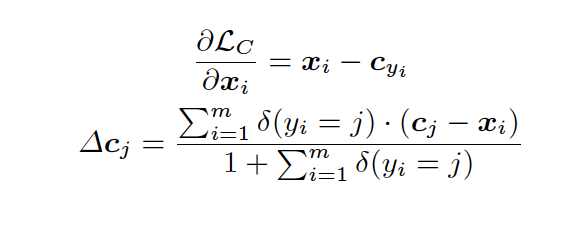
\includegraphics[width=0.4\textwidth]{gradient.png}\\
%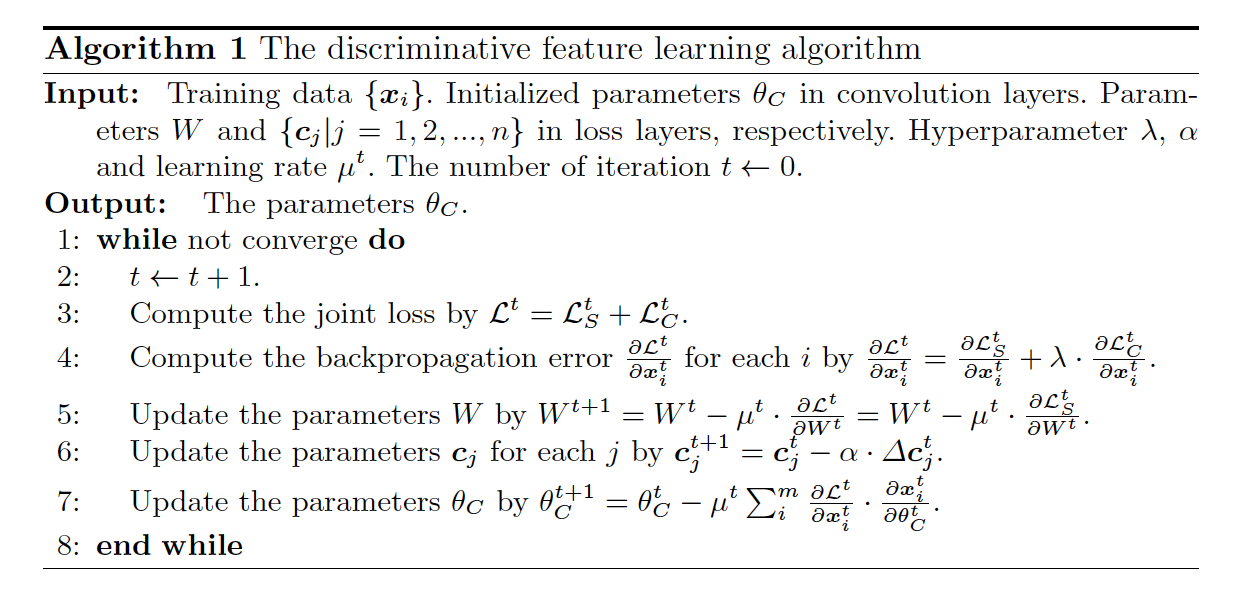
\includegraphics[width=0.9\textwidth]{algrothem.png}\\
%\end{tabular}
%\end{center}
%\end{table}

We use the same parameter settings as in Section~\ref{subsec:primary_result}, with $\lambda = 0.03$. Unfortunately, only adding a Center Loss function does not improve the detection performance. One possible reason might be that while minimizing the intra-class variance, the Center Loss function also decreases the distances among centers. Figures~\ref{fig:center_loss_failure} presents the value of the center loss function along with the sum of all distances between each deep feature and its non-corresponding centers during Stage $2$: Fast-RCNN training. It is observed that when we decrease the center loss, the sum of distances is also reduced to only $20$ to $30$. However, this value is more than $1000$ in the original Faster-RCNN. 

Since the difference in deep features for police and others is initially small, when the centers become close to each other, they may be more difficult to distinguish, therefore impairing the detection ability. However, we cannot simply abandon the Center Loss because huge intra-variance exists in the case of the \textit{others} class. To increase the mAP, it is necessary to have Center Loss in our total loss function with more modification.
\begin{figure}[H]
\centering
\begin{minipage}{\textwidth} % choose width suitably
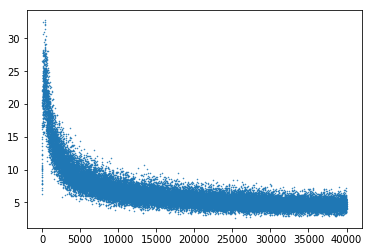
\includegraphics[width=0.5\textwidth]{center_2.png}
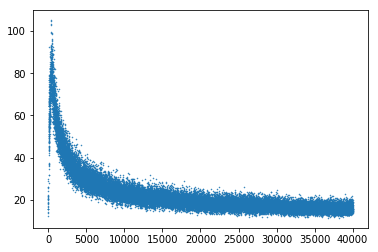
\includegraphics[width=0.5\textwidth]{sum_of_dot_2.png}\\
\footnotesize{The left figure presents the value of center loss function during the Stage $2$ Fast-RCNN training, in which x-axis shows the step; the right figure presents the sum of all distances between each deep feature and its non-corresponding centers during the Stage $2$ Fast-RCNN training. \par}
\end{minipage}
\caption{Training Value with Center Loss function}
\label{fig:center_loss_failure}
\end{figure}

\subsection{Contrastive Loss}
The previous result, along with many other experiments, shows us a positive correlation between inter-class distance and intra-class distance. However, in our case we need to make them compete with each other and make a balance, staying in a reasonable interval. Therefore, we try to introduce the Contrastive Loss function to balance the effect of the center loss function.. 

The first Contrastive Loss that we propose is 
\begin{equation}
	\mathcal{L}_{ct} = - \sum_{\substack{i,j \in N \\ i \neq j}} \Vert \mathbf{c}_{i} - \mathbf{c}_{j} \Vert^{2}
\end{equation}
where $N$ specifies the number of total classes. And the overall loss function becomes
\begin{equation}
		\mathcal{L}  = \mathcal{L}_{s} + \frac{\lambda}{2} \mathcal{L}_{c} + \frac{\mu}{2} \mathcal{L}_{ct}
\end{equation}
where $\lambda$ is the weight of the Center Loss and $\mu$ is the weight of the Contrastive Loss.

We try the same experiment, but the program does not perform very well, as the Center Loss is dominated by the Contrastive Loss, leading to an extremely large center distance. Another problem with this design is the way we update the parameters. We use SGD to update both centers and features with respect to the Center Loss \footnote{The update formula is shown in Equation~\ref{eqn:center_gradient}.}. However, our Contrastive Loss is merely a function of centers; its gradient with respect to $x$ is $0$ and thus this function does not help backpropagate $x$. This may lead to a problem of mismatch between features and their center. 

To fix these problems, we use another form of the Contrastive Loss, which maximizes the distance between deep features and the other class centers. An upper bound is also added to prevent divergence.
\begin{equation}
	\mathcal{L}_{new-ct} = [\text{Constant} - \sum_{\substack{i,j \in m \\ y_i \neq y_j}} \Vert \mathbf{x}_{i} - \mathbf{c}_{ y_{j}} \Vert^{2},0]_{+}
\end{equation}
where $m$ specifies the size of the mini-batch. Our total loss function becomes
\begin{equation}
	\mathcal{L}  = \mathcal{L}_{s} + \frac{\lambda}{2} \mathcal{L}_{c} + \frac{\mu}{2} \mathcal{L}_{new-ct}
\end{equation}
where $\lambda$ is the weight of the Center Loss and $\mu$ is the weight of the Contrastive Loss.

\begin{figure}[H]
\centering
\begin{minipage}{\textwidth} % choose width suitably
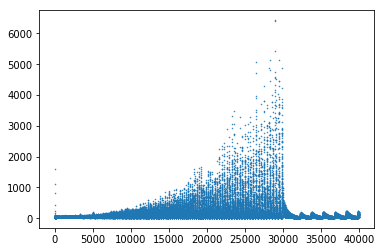
\includegraphics[width=0.5\textwidth]{center_l2.png}
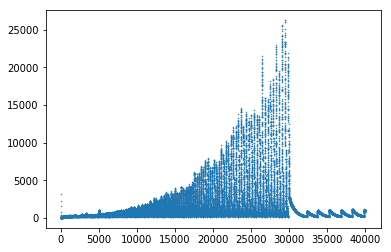
\includegraphics[width=0.5\textwidth]{sum_of_dot_1.png}\\
\footnotesize{The left figure presents the value of center loss function during the Stage $2$ Fast-RCNN training, in which x-axis shows the step ; the right figure presents the sum of distances between each deep feature and its non-corresponding centers during the Stage $2$ Fast-RCNN training. We do the experiment with the same parameter setting as the original model, with $\lambda = 0.003, \mu = 0.00003, \text{Constant} = 200$ \par}
\end{minipage}
\caption{Intra-class and Inter-class Center Distance}
\label{fig:contrasive_1}
\end{figure}

\begin{figure}[H]
\centering
\begin{minipage}{\textwidth} % choose width suitably
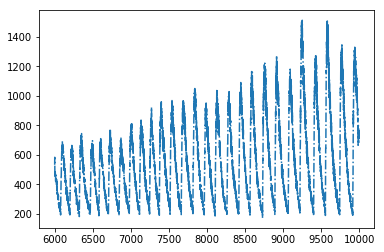
\includegraphics[width=0.5\textwidth]{head.png}
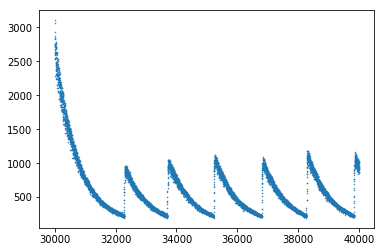
\includegraphics[width=0.5\textwidth]{tail.png}\\
\footnotesize{The left figure presents the sum of distances between each deep feature and its non-corresponding centers during the Stage $2$ Fast-RCNN training between Step $6000-10000$ ; the right figure presents the sum of distances between each deep features and their non-corresponding centers during the Stage $2$ Fast-RCNN training between Step $30000-40000$. We do the experiment with the same parameter setting as the original model, with $\lambda = 0.003, \mu = 0.00003, \text{Constant} = 200$ \par}
\end{minipage}
\caption{Inter-class Center Distance in Detail}
\label{fig:contrasive_2}
\end{figure}

In the experiment result, we do see a balance between the two loss functions. Figure~\ref{fig:contrasive_1} shows that the fluctuation in the inter-class and intra-class distances becomes larger when we continue training. However, after 30000 iterations when we half the learning rate, the fluctuation goes down, but there is still the tendency for the peak of loss to grow. 

Figure~\ref{fig:contrasive_2} presents the inter-class center distance in detail. For instance, from 6000 iterations to 10000 iterations, when the Contrastive Loss is non-zero, both inter-class and intra-class distances exhibit a quick increase followed by a tendency to decrease until Contrastive Loss is activated again.

Up to this point, our results show instability so we are still working on testing different parameters and trying other forms of loss functions.


\section{Conclusion and Future Work}

In this work, we have applied Faster-RCNN to the problem of police detection in body-worn video with good initial results. We have demonstrated multiple approaches to improve the performance of the network: We have modified the loss function to utilize center loss and contrastive loss, and we have performed enhancement techniques on the images. Changing the loss functions has not yet produced satisfactory results, but we have made a lot of progress in finding a better loss function. We have also enhanced all of the images, which will likely improve the quality of detection.

Looking into the future, we still have many ways to improve these results. We can determine the ideal parameters of loss functions to improve detection ability, and we can do further research on the appropriate loss function to use. Expanding outside of the realm of object detection, we have begun work on using semantic analysis to extract information from the audio in the video, and we would like to develop an object tracking algorithm for body-worn video. We look forward to both constructing a better object detection algorithm and using that knowledge in related fields.

\section*{Acknowledgements}
We are very grateful for the help of our postdoctoral mentor, Professor Bao Wang, and faculty mentors Andrea Bertozzi and Jeffrey Brantingham. Our work was possible thanks to the UCLA Computational Research Training Program in Computational and Applied Mathematics, with funding from the National Science Foundation Grant DMS-1045536. We also thank the Los Angeles Police Department for supplying the video data for the project.

\maketitle
\nocite{*}
\bibliographystyle{plain}
\bibliography{annot}

\end{document}